\let\negmedspace\undefined
\let\negthickspace\undefined
\documentclass[journal,12pt,onecolumn]{IEEEtran}
\usepackage{cite}
\usepackage{amsmath,amssymb,amsfonts,amsthm}
\usepackage{algorithmic}
\usepackage{graphicx}
\graphicspath{{./figs/}}
\usepackage{textcomp}
\usepackage{xcolor}
\usepackage{txfonts}
\usepackage{listings}
\usepackage{enumitem}
\usepackage{mathtools}
\usepackage{gensymb}
\usepackage{comment}
\usepackage{caption}
\usepackage[breaklinks=true]{hyperref}
\usepackage{tkz-euclide} 
\usepackage{listings}
\usepackage{gvv}                                        
%\def\inputGnumericTable{}                                 
\usepackage[latin1]{inputenc}     
\usepackage{xparse}
\usepackage{color}                                            
\usepackage{array}                                            
\usepackage{longtable}                                       
\usepackage{calc}                                             
\usepackage{multirow}
\usepackage{multicol}
\usepackage{hhline}                                           
\usepackage{ifthen}                                           
\usepackage{lscape}
\usepackage{tabularx}
\usepackage{array}
\usepackage{float}
\newtheorem{theorem}{Theorem}[section]
\newtheorem{problem}{Problem}
\newtheorem{proposition}{Proposition}[section]
\newtheorem{lemma}{Lemma}[section]
\newtheorem{corollary}[theorem]{Corollary}
\newtheorem{example}{Example}[section]
\newtheorem{definition}[problem]{Definition}
\newcommand{\BEQA}{\begin{eqnarray}}
\newcommand{\EEQA}{\end{eqnarray}}
\newcommand{\define}{\stackrel{\triangle}{=}}
\theoremstyle{remark}
\newtheorem{rem}{Remark}

\begin{document}
\title{
ASSIGNMENT 3: GATE 2016 \\
     PH:PHYSICS}
\author{AI25BTECH11035 - Sujal Rajani }
\maketitle
\renewcommand{\thefigure}{\theenumi}
\renewcommand{\thetable}{\theenumi}

\begin{enumerate}

\item The volume of a sphere of diameter 1 unit is \_\_\_\_\_\_\_\_\_ than the volume of a cube of side 1 unit.
\begin{multicols}{4}
\begin{enumerate}
    \item least
    \item less
    \item lesser
    \item low
\end{enumerate}
\end{multicols}

\item The unruly crowd demanded that the accused be \_\_\_\_\_\_\_\_\_\_\_ without trial.
\begin{multicols}{4}
\begin{enumerate}
    \item hanged
    \item hanging
    \item hankering
    \item hung
\end{enumerate}
\end{multicols}

\item Choose the statement(s) where the underlined word is used correctly:

(i) A \underline{pronc} is a dried plum. 
(ii)He was lying \underline{prone} on the floor. 
(iii) People who eat a lot of fat are \underline{prone} to heart disease.


\begin{multicols}{4}
\begin{enumerate}
    \item (i) and (iii) only
    \item (iii) only
    \item (i) and (ii) only
    \item (ii) and (iii) only
\end{enumerate}
\end{multicols}

\item \textbf{Fact:} If it rains, then the field is wet.

Read the following statements: 
(i) It rains
(ii) The field is not wet
(iii) The field is wet
(iv) It did not rain
Which one of the options given below is \textbf{NOT} logically possible, based on the given fact?
\begin{multicols}{2}
\begin{enumerate}
    \item If (iii), then (iv).
    \item If (i), then (iii).
    \item If (i), then (ii).
    \item If (ii), then (iv).
\end{enumerate}
\end{multicols}

\item A window is made up of a square portion and an equilateral triangle portion above it. The base of the triangular portion coincides with the upper side of the square. If the perimeter of the window is 6 m, the area of the window in m$^2$ is \_\_\_\_\_\_.
\begin{multicols}{4}
\begin{enumerate}
    \item 1.43
    \item 2.06
    \item 2.68
    \item 2.88
\end{enumerate}

\end{multicols}
\textbf{Q6-Q10 carry two marks each}
\item Students taking an exam are divided into two groups, \textbf{ P } and \textbf{ Q } such that each group has the same number of students. The performance of each of the students in a test was evaluated out of 200 marks. It was observed that the mean of group \textbf{P} was 105, while that of group \textbf{Q} was 85. The standard deviation of group \textbf{P} was 25, while that of group \textbf{Q} was 5. Assuming that the marks were distributed on a normal distribution, which of the following statements will have the highest probability of being \textbf{TRUE}?


\begin{enumerate}
    \item No student in group \textbf{Q} scored less marks than any student in group \textbf{P}.
    \item No student in group \textbf{P} scored less marks than any student in group \textbf{Q}.
    \item Most students of group \textbf{Q} scored marks in a narrower range than students in group \textbf{P}.
    \item The median of the marks of group \textbf{P} is 100.
\end{enumerate}


\item A smart city integrates all modes of transport, uses clean energy and promotes sustainable use of resources. It also uses technology to ensure safety and security of the city, something which critics argue, will lead to a surveillance state.

Which of the following can be logically inferred from the above paragraph?

(i) All smart cities encourage the formation of surveillance states.
(ii) Surveillance is an integral part of a smart city.
(iii) Sustainability and surveillance go hand in hand in a smart city.
(iv) There is a perception that smart cities promote surveillance.

\begin{multicols}{2}
\begin{enumerate}
    \item (i) and (iv) only
    \item (ii) and (iii) only
    \item (iv) only
    \item (i) only
\end{enumerate}
\end{multicols}


\item Find the missing sequence in the letter series.
B, HH, LNP, \_\_\_\_. 

\begin{multicols}{4}
\begin{enumerate}
    \item SUWY
    \item TUVW
    \item TVXZ
    \item TWXZ
\end{enumerate}
\end{multicols}


\item The binary operation $\square$ is defined as $a \square b = ab +(a+b)$, where $a$ and $b$ are any two real numbers. The value of the identity element of this operation, defined as the number $x$ such that $a \square x = a$, for any $a$, is \_\_\_\_\_.
\begin{multicols}{2}
\begin{enumerate}
    \item 0
    \item 1
    \item 2
    \item 10
\end{enumerate}
\end{multicols}
\item Which of the follofwing curves respresents the abscissa and y represents the funtion y = $ln(|e6^{[|\sin(|x|)|]}|)$ for $|x|$<2$\pi$ ?
Here,  $x$ represent the abscissa and y represents the ordinate.
\begin{figure}[H]
    \centering
    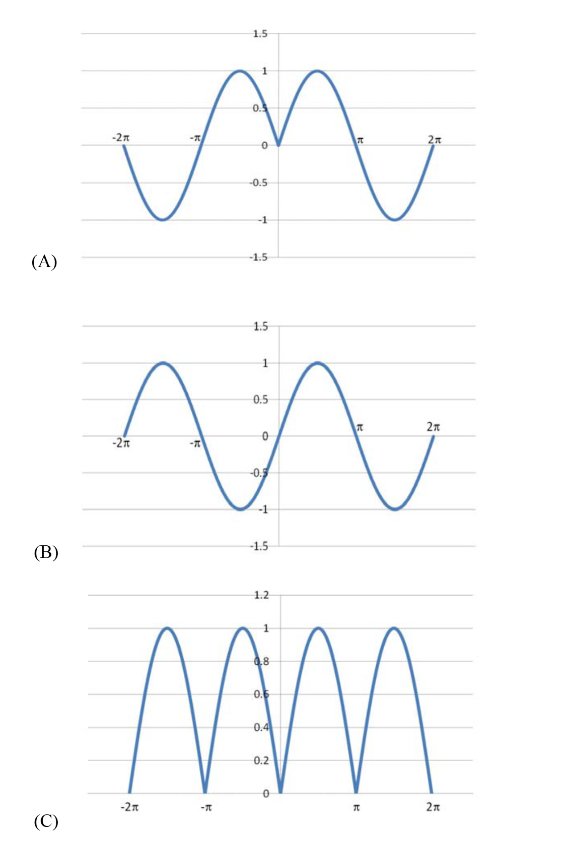
\includegraphics[width = 0.3\columnwidth]{fig/Q10(1).png}
    \caption*{}
    \label{fig:Q10(1)}
\end{figure}
\begin{figure}[H]
    \centering
    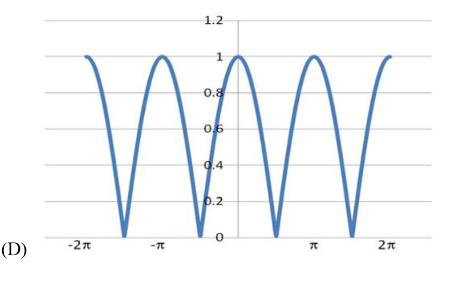
\includegraphics[width = 0.2\columnwidth]{fig/Q10(2).png}
    \caption*{}
    \label{fig:Q10(2)}
\end{figure}
\end{enumerate}
\section*{\textbf{END OF THE QUESTION PAPER} }

\newpage
\textbf{Q1-Q25 carry one mark each}
\begin{enumerate}


\item Consider the linear differential equation $\dfrac{dy}{dx} = xy$. If $y = 2$ at $x = 0$, then the value of $y$ at $x = 2$ is given by

\begin{multicols}{2}
\begin{enumerate}
    \item $e^{-2}$
    \item $2e^{-2}$
    \item $e^{2}$
    \item $2e^{2}$
\end{enumerate}
\end{multicols}

\item Which of the following magnetic vector potentials gives rise to a uniform magnetic field $\vec{B}_0 \hat{k}$?
\begin{multicols}{2}
\begin{enumerate}
    \item $B_0 z \hat{k}$
    \item $-B_0 x \hat{j}$
    \item $\dfrac{B_0}{2}
    (-y\hat{i} + x\hat{j})$
    \item $\dfrac{B_0}{2}
    (y\hat{i} + x\hat{j})$
\end{enumerate}
\end{multicols}

\item The molecule $^{17}O_{2}$ is
\begin{enumerate}
    \item Raman active but not NMR (nuclear magnetic resonance) active.
    \item Infrared active and Raman active but not NMR active.
    \item Raman active and NMR active.
    \item Only NMR active.
\end{enumerate}

\item There are four electrons in the $3d$ shell of an isolated atom. The total magnetic moment of the atom in units of Bohr magneton is \underline{\hspace{2cm}}.

\item Which of the following transitions is NOT allowed in the case of an atom, according to the electric dipole radiation selection rule?
\begin{multicols}{4}
\begin{enumerate}
    \item 2s-1s
    \item 2p-1s
    \item 2p-2s
    \item 3d-2p
\end{enumerate}
\end{multicols}

\item In the SU(3) quark model, the triplet of mesons $(\pi^{+}, \pi^{0}, \pi^{-})$ has
\begin{enumerate}
    \item Isospin = 0, Strangeness = 0
    \item Isospin = 1, Strangeness = 0
    \item Isospin = 1/2, Strangeness = +1
    \item Isospin = 1/2, Strangeness = -1
\end{enumerate}

\item The magnitude of the magnetic dipole moment associated with a square shaped loop carrying a steady current $I$ is $m$. If this loop is changed to a circular shape with the same current $I$ passing through it, the magnetic dipole moment becomes $\dfrac{ \rho m}{\pi}$. The value of $\rho$ is \underline{\hspace{2cm}}.

\item The total power emitted by a spherical black body of radius $R$ at a temperature $T$ is $P_1$. Let $P_2$ be the total power emitted by another spherical black body of radius $R/2$ kept at temperature $2T$. The ratio, $P_1/P_2$ is \underline{\hspace{2cm}}. (Give your answer up to two decimal places.)

\item The entropy $S$ of a system of $N$ spins, which may align either in the upward or in the downward direction, is given by $S = -k_b N [ p \ln p + (1 - p) \ln (1 - p) ]$. Here $k_b$ is the Boltzmann constant. The probability of alignment in the upward direction is $p$. The value of $p$, at which the entropy is maximum, is \underline{\hspace{2cm}}. (Give your answer upto one decimal place)

\item For a system at constant temperature and volume, which of the following statements is correct at equilibrium?


\begin{enumerate}
    \item The Helmholtz free energy attains a local minimum.
    \item The Helmholtz free energy attains a local maximum.
    \item The Gibbs free energy attains a local minimum.
    \item The Gibbs free energy attains a local maximum.
\end{enumerate}


\item $N$ atoms of an ideal gas are enclosed in a container of volume $V$. The volume of the container is changed to $4V$, while keeping the total energy constant. The change in the entropy of the gas, in units of $N k_b \ln 2$, is \underline{\hspace{2cm}}, where $k_b$ is the Boltzmann constant.

\item Which of the following is an analytic function of $z$ everywhere in the complex plane?

\begin{multicols}{4}
\begin{enumerate}
    \item $z^2$
    \item $(z^*)^2$
    \item $|z|^2$
    \item $\sqrt{z}$
\end{enumerate}
\end{multicols}

\item In a Young's double slit experiment using light, the apparatus has two slits of unequal widths. When only slit-1 is open, the maximum observed intensity on the screen is $4I_0$. When only slit-2 is open, the maximum observed intensity is $I_0$. When both slits are open, an interference pattern appears on the screen. The ratio of the intensity of the principal maximum to that of the nearest minimum is \underline{\hspace{2cm}}.

\item Consider a metal which obeys the Sommerfeld model exactly. If $E_F$ is the Fermi energy of the metal at $T = 0$ K and $R_H$ is its Hall coefficient, which of the following statements is correct?

\begin{multicols}{4}
\begin{enumerate}
    \item $R_H \propto {E_F}^{3/2}$
    \item $R_H \propto {E_F}^{2/3}$
    \item $R_H \propto {E_F}^{-3/2}$
    \item $R_H$ is independent of $E_F$
\end{enumerate}
\end{multicols}

\item A one-dimensional linear chain of atoms contains two types of atoms of masses $m_1$ and $m_2$ ($m_2 > m_1$), arranged alternately. The distance between successive atoms is the same. Assume that the harmonic approximation is valid. At the first Brillouin zone boundary, which of the following statements is correct?

\begin{enumerate}
    \item The atoms of mass $m_2$ are at rest in the optical mode, while they vibrate in the acoustical mode.
    \item The atoms of mass $m_1$ are at rest in the optical mode, while they vibrate in the acoustical mode.
    \item Both types of atoms vibrate with equal amplitudes in the optical as well as in the acoustical modes.
    \item Both types of atoms vibrate, but with unequal, non-zero amplitudes in the optical as well as in the acoustical modes.
\end{enumerate}

\item Which of the following operators is Hermitian?

\begin{multicols}{4}
\begin{enumerate}
    \item $\dfrac{d}{dx}$
    \item $\dfrac{d^2}{dx^2}$
    \item $i\dfrac{d^2}{dx^2}$
    \item $\dfrac{d^3}{dx^3}$
\end{enumerate}
\end{multicols}


\item The kinetic energy of a particle of rest mass $m_0$ is equal to its rest mass energy. Its momentum in units of $m_0c$, where $c$ is the speed of light in vacuum, is \underline{\hspace{2cm}}. (Give your answer upto two decimal places)

\item The number density of electrons in the conduction band of a semiconductor at a given temperature is $2 \times 10^{19}~\mathrm{m}^{-3}$. Upon lightly doping this semiconductor with donor impurities, the number density of conduction electrons at the same temperature becomes $4 \times 10^{20}~\mathrm{m}^{-3}$. The ratio of majority to minority charge carrier concentration is \underline{\hspace{2cm}}.

\item Two blocks are connected by a spring of spring constant $k$. One block has mass $m$ and the other block has mass $2m$. If the ratio $k/m = 4~\mathrm{s}^{-2}$, the angular frequency of vibration $\omega$ of the two block spring system in $\mathrm{s}^{-1}$ is \underline{\hspace{2cm}}. (Give your answer upto two decimal places)

\item A particle moving under the influence of a central force $\vec{F}(r) = -k\vec{r}$ (where $\vec{r}$ is the position vector of the particle and $k$ is a positive constant) has non-zero angular momentum. Which of the following curves is a possible orbit for this particle?

\begin{enumerate}
    \item A straight line segment passing through the origin.
    \item An ellipse with its center at the origin.
    \item An ellipse with one of the foci at the origin.
    \item A parabola with its vertex at the origin.

\end{enumerate}
    


\item Consider the reaction $
^{54}_{25}\mathrm{Mn} + e^- \longrightarrow ^{54}_{24}\mathrm{Cr} + X
$. The particle $X$ is

\begin{multicols}{4}
\begin{enumerate}
    \item $\gamma$
    \item $\nu_e$
    \item $n$
    \item $\pi^0$
\end{enumerate}
\end{multicols}

\item The scattering of particles by a potential can be analyzed by Born approximation. In particular, if the scattered wave is replaced by an appropriate plane wave, the corresponding Born approximation is known as the first Born approximation. Such an approximation is valid for


\begin{enumerate}
    \item Large incident energies and weak scattering potentials.
    \item Large incident energies and strong scattering potentials.
    \item Small incident energies and weak scattering potentials.
    \item Small incident energies and strong scattering potentials.
\end{enumerate}


    



\item Consider an elastic scattering of particles in $l=0$ states. If the corresponding phase shift $\delta_0$ is $90^\circ$ and the magnitude of the incident wave vector is equal to $\sqrt{2\pi}$~fm$^{-1}$, then the total scattering cross section in units of fm$^2$ is \underline{\hspace{2cm}}.

\item A hydrogen atom is in its ground state. In the presence of a uniform electric field $\vec{E}=E_0\hat{z}$, the leading order change in its energy is proportional to $(E_0)^n$. The value of the exponent $n$ is \underline{\hspace{2cm}}.




\item A solid material is found to have a temperature independent magnetic susceptibility, $\chi = C$. Which of the following statements is correct?

\begin{enumerate}
    \item If $C$ is positive, the material is a diamagnet.
    \item If $C$ is positive, the material is a ferromagnet.
    \item If $C$ is negative, the material could be a type I superconductor.
    \item If $C$ is positive, the material could be a type I superconductor.
\end{enumerate}



\textbf{Q.26 -- Q.55 carry two marks each.}

\item An infinite, conducting slab kept in a horizontal plane carries a uniform charge density $\sigma$. Another infinite slab of thickness $t$, made of a linear dielectric material of dielectric constant $k$, is kept above the conducting slab. The bound charge density on the upper surface of the dielectric slab is

\begin{multicols}{2}
\begin{enumerate}
    \item $\dfrac{\sigma}{2k}$
    \item $\dfrac{\sigma}{k}$
    \item $\dfrac{\sigma (k - 2)}{2k}$
    \item $\dfrac{\sigma (k - 1)}{k}$
\end{enumerate}
\end{multicols}

\item The number of spectroscopic terms resulting from the $\vec{L} \cdot \vec{S}$ coupling of a $3p$ electron and a $3d$ electron is \underline{\hspace{2cm}}.

\item Which of the following statements is NOT correct?

\begin{enumerate}
    \item A deuteron can be disintegrated by irradiating it with gamma rays of energy 4 MeV.
    \item A deuteron has no excited states.
    \item A deuteron has no electric quadrupole moment.
    \item The $^1S_0$ state of deuteron cannot be formed.
\end{enumerate}

\item If $\vec{S}_1$ and $\vec{S}_2$ are the spin operators of the two electrons of a He atom, the value of $\langle \vec{S}_1 \cdot \vec{S}_2 \rangle$ for the ground state is

\begin{multicols}{4}
\begin{enumerate}
    \item $-\dfrac{3}{2}\hbar^2$
    \item $-\dfrac{3}{4}\hbar^2$
    \item $0$
    \item $\dfrac{1}{4}\hbar^2$
\end{enumerate}
\end{multicols}

\item A two-dimensional square rigid box of side $L$ contains six non-interacting electrons at $T=0$ K. The mass of the electron is $m$. The ground state energy of the system of electrons, in units of $\dfrac{\pi^2\hbar^2}{2mL^2}$, is \underline{\hspace{2cm}}.

\item An alpha particle is accelerated in a cyclotron. It leaves the cyclotron with a kinetic energy of $16$ MeV. The potential difference between the D electrodes is $50$ kilovolts. The number of revolutions the alpha particle makes in its spiral path before it leaves the cyclotron is \underline{\hspace{2cm}}.


\item Let $V_i$ be the $i$th component of a vector field $\vec{V}$, which has zero divergence. If $\partial_j \equiv \partial / \partial x_j$, the expression for $\epsilon_{ijk} \partial_j \partial_l V_m$ is equal to

\begin{multicols}{4}
\begin{enumerate}
    \item $-\partial_j \partial_k V_i$
    \item $\partial_j \partial_k V_i$
    \item $\partial^2_j V_i$
    \item $-\partial^2_j V_i$
\end{enumerate}
\end{multicols}

\item The direction of $\vec{\nabla} f$ for a scalar field $f(x, y, z) = \frac{1}{2}x^2 - xy + \frac{1}{2}z^2$ at the point $P(1, 1, 2)$ is

\begin{multicols}{4}
\begin{enumerate}
    \item $\dfrac{(-\hat{j} - 2\hat{k})}{\sqrt{5}}$
    \item $\dfrac{(-\hat{j} + 2\hat{k})}{\sqrt{5}}$
    \item $\dfrac{(\hat{j} - 2\hat{k})}{\sqrt{5}}$
    \item $\dfrac{(\hat{j} + 2\hat{k})}{\sqrt{5}}$
\end{enumerate}
\end{multicols}

\item $\sigma_x$, $\sigma_y$, and $\sigma_z$ are the Pauli matrices. The expression $2 \sigma_x \sigma_y + \sigma_y \sigma_x$ is equal to

\begin{multicols}{4}
\begin{enumerate}
    \item $-3i\sigma_z$
    \item $-i\sigma_z$
    \item $i\sigma_z$
    \item $3i\sigma_z$
\end{enumerate}
\end{multicols}

\item A particle of mass $m = 0.1$~kg is initially at rest at origin. It starts moving with a uniform acceleration $\vec{a} = 10\hat{i}$~m~s$^{-2}$ at $t = 0$. The action $S$ of the particle, in units of J-s, at $t = 2$s is \underline{\hspace{2cm}}. (Give your answer up to two decimal places.)

\item A periodic function $f(x)$ of period $2\pi$ is defined in the interval $(-\pi < x < \pi)$ as:
$
f(x) =
\begin{cases}
-1, -\pi < x < 0 \\
1,  0 < x < \pi
\end{cases}
$
The appropriate Fourier series expansion for $f(x)$ is


\begin{enumerate}
    \item $f(x) = (4/\pi)[\sin x + (\sin 3x)/3 + (\sin 5x)/5 + \cdots ]$
    \item $f(x) = (4/\pi)[\sin x - (\sin 3x)/3 + (\sin 5x)/5 - \cdots ]$
    \item $f(x) = (4/\pi)[\cos x + (\cos 3x)/3 + (\cos 5x)/5 + \cdots ]$
    \item $f(x) = (4/\pi)[\cos x - (\cos 3x)/3 + (\cos 5x)/5 - \cdots ]$
\end{enumerate}


\item Atoms, which can be assumed to be hard spheres of radius $R$, are arranged in an fcc lattice with lattice constant $a$, such that each atom touches its nearest neighbours. Take the center of one of the atoms as the origin. Another atom of radius $r$ (assumed to be hard sphere) is to be accommodated at a position $(0, a/2, 0)$ without distorting the lattice. The maximum value of $r/R$ is \underline{\hspace{2cm}}. (Give your answer up to two decimal places.)

\item In an inertial frame of reference $S$, an observer finds two events occurring at the same time at coordinates $x_1 = 0$ and $x_2 = d$. A different inertial frame $S'$ moves with velocity $v$ with respect to $S$ along the positive x-axis. An observer in $S'$ also notices these two events and finds them to occur at times $t_1'$ and $t_2'$ and at positions $x_1'$ and $x_2'$, respectively. If $\Delta t' = t_2' - t_1'$, $\Delta x' = x_2' - x_1'$ and $\gamma = \dfrac{1}{\sqrt{1-\dfrac{v^2}{c^2}}}$, which of the following statements is true?

\begin{multicols}{2}
\begin{enumerate}
    \item $\Delta t' = 0, \Delta x' = \gamma d$
    \item $\Delta t' = 0, \Delta x' = d/\gamma$
    \item $\Delta t' = -\gamma v d / c^2, \Delta x' = \gamma d$
    \item $\Delta t' = -\gamma v d / c^2, \Delta x' = d/\gamma$
\end{enumerate}
\end{multicols}

\item The energy vs. wave vector $(E - k)$ relationship near the bottom of a band for a solid can be approximated as $E = A (ka)^2 + B (ka)^4$, where the lattice constant $a = 2.1A$. The values of $A$ and $B$ are $6.3 \times 10^{-19}$J and $3.2 \times 10^{-20}$J, respectively. At the bottom of the conduction band, the ratio of the effective mass of the electron to the mass of free electron is \underline{\hspace{2cm}}. (Give your answer upto two decimal places)\\
(Take $\hbar = 1.05 \times 10^{-34}$J-s, mass of free electron $= 9.1 \times 10^{-31}$kg)

\item The electric field component of a plane electromagnetic wave travelling in vacuum is given by $\vec{E}(z, t) = E_0 \cos(kz - \omega t) \hat{i}$. The Poynting vector for the wave is


\begin{enumerate}
    \item $(c \epsilon_0  /2)E^2 \cos^2 (kz - \omega t) \hat{j}$
    \item $(c \epsilon_0  /2)E_0^2 \cos^2 (kz - \omega t) \hat{k}$
    \item $c \epsilon_0 E_0^2 \cos^2 (kz - \omega t) \hat{j}$
    \item $c \epsilon_0 E_0^2 \cos^2 (kz - \omega t) \hat{k}$
\end{enumerate}

    \item Consider a system having three energy levels with energies $0$, $2\epsilon$ and $3\epsilon$, with respective degeneracies of $2$, $2$ and $3$. Four bosons of spin zero have to be accommodated in these levels such that the total energy of the system is $10\epsilon$. The number of ways in which it can be done is \underline{\hspace{2cm}}.
    \newpage
    \item The Lagrangian of a system is given by
    $
L = \frac{1}{2} m l^2 \sbrak{\dot{\theta}^2 + \sin^2 \theta\, \dot{\phi}^2 }\ - mgl \cos \theta $, where $m$, $l$ and $g$ are constants .\\
    Which of the following is conserved?
    \begin{multicols}{4}
    \begin{enumerate}
        \item $\dot{\phi}\sin^2 \theta$
        \item $\dot{\phi}\sin \theta$
        \item $\dfrac{\dot{\phi}}{\sin\theta}$
        \item $\dfrac{\dot{\phi}}{\sin^2\theta}$
    \end{enumerate}
    \end{multicols}
    
    \item Protons and $\alpha$-particles of equal initial momenta are scattered off a gold foil in a Rutherford scattering experiment. The scattering cross sections for proton on gold and $\alpha$-particle on gold are $\sigma_p$ and $\sigma_{\alpha}$ respectively. The ratio $\sigma_{\alpha}/\sigma_{p}$ is \underline{\hspace{2cm}}.
    
    \item For the digital circuit given below, the output $X$ is
    \begin{figure}[H]
    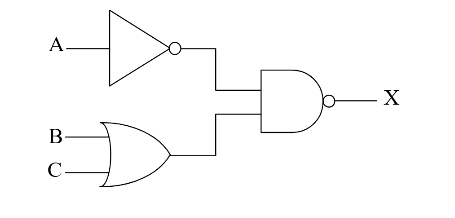
\includegraphics[width = 0.5\columnwidth]{fig/Q44.png}
    \centering
    \caption*{}
    \label{fig:Q44}
\end{figure}
\begin{enumerate}
\begin{multicols}{2}
    
    \item $\overline{\overline{\text{A}} + \text{B} \cdot \text{C}}$
    \item $\overline{\overline{\text{A}} \cdot (\text{B} + \text{C})}$
     \item $\overline{\text{A}} \cdot (\text{B} + \text{C})$
    \item $\text{A} + \overline{\text{B} \cdot \text{C}}$ 
    \end{multicols}
    \end{enumerate}
    
    \item The Fermi energies of two metals $X$ and $Y$ are $5\,\textrm{eV}$ and $7\,\textrm{eV}$ and their Debye temperatures are $170\,\textrm{K}$ and $340\,\textrm{K}$, respectively. The molar specific heats of these metals at constant volume at low temperatures can be written as $(C_V)_X = \gamma_X T + A_X T^3$ and $(C_V)_Y = \gamma_Y T + A_Y T^3$, where $\gamma$ and $A$ are constants. Assuming that the thermal effective mass of the electrons in the two metals are same, which of the following is correct?
    
    \begin{multicols}{2}
    \begin{enumerate}
        \item $\dfrac{\gamma_X}{\gamma_Y} = \dfrac{7}{5}, \quad \dfrac{A_X}{A_Y} = 8$
        \item $\dfrac{\gamma_X}{\gamma_Y} = \dfrac{7}{5}, \quad \dfrac{A_X}{A_Y} = \dfrac{1}{8}$
        \item $\dfrac{\gamma_X}{\gamma_Y} = \dfrac{5}{7}, \quad \dfrac{A_X}{A_Y} = \dfrac{1}{8}$
        \item $\dfrac{\gamma_X}{\gamma_Y} = \dfrac{5}{7}, \quad \dfrac{A_X}{A_Y} = 8$
    \end{enumerate}
    \end{multicols}
    
    \item A two-level system has energies zero and $E$. The level with zero energy is non-degenerate, while the level with energy $E$ is triply degenerate. The mean energy of a classical particle in this system at a temperature $T$ is
    \begin{multicols}{2}
    \begin{enumerate}
        \item $\dfrac{E e^{-E/k_B T}}{1 + 3 e^{-E/k_B T}}$
        \item $\dfrac{E e^{-E/k_B T}}{1 + e^{-E/k_B T}}$
        \item $\dfrac{3 E e^{-E/k_B T}}{1 + 3 e^{-E/k_B T}}$
        \item $\dfrac{3 E e^{-E/k_B T}}{1 + e^{-E/k_B T}}$
    \end{enumerate}
    \end{multicols}
    
    \item A particle of rest mass $M$ is moving along the positive $x$-direction. It decays into two photons $\gamma_1$ and $\gamma_2$, as shown in the figure. The energy of $\gamma_1$ is $1\,\text{GeV}$ and the energy of $\gamma_2$ is $0.82\,\text{GeV}$. The value of $M$ (in units of GeV/$c^2$) is \underline{\hspace{2cm}}. (Give your answer up to two decimal places)
   \begin{figure}[H]
    \centering
    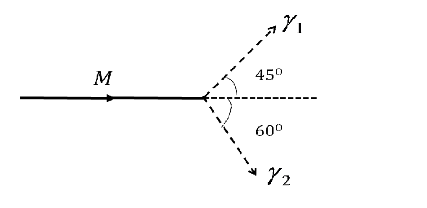
\includegraphics[width = 0.5\columnwidth]{fig/Q47.png}
    \caption*{}
    \label{fig:Q47}
\end{figure}
    \item If $x$ and $p$ are the $x$ components of the position and the momentum operators of a particle respectively, the commutator $[x^2, p^2]$ is
    \begin{enumerate}
        \item $i\hbar (xp - px)$
        \item $2i\hbar (xp - px)$
        \item $i\hbar (xp + px)$
        \item $2i\hbar (xp + px)$
    \end{enumerate}
    
    \item The $x$-$y$ plane is the boundary between free space and a magnetic material with relative permeability $\mu_r$. The magnetic field in the free space is $B_x \hat{i} + B_z \hat{k}$. The magnetic field in the magnetic material is
    \begin{enumerate}
        \item $B_x \hat{i} + B_z \hat{k}$
        \item $B_x \hat{i} + \mu_r B_z \hat{k}$
        \item $\dfrac{1}{\mu_r} B_x \hat{i} + B_z \hat{k}$
        \item $\mu_r B_x \hat{i} + B_z \hat{k}$
    \end{enumerate}
    
    \item Let $|l, m\rangle$ be the simultaneous eigenstates of $L^2$ and $L_z$. Here $\vec{L}$ is the angular momentum operator with Cartesian components $(L_x, L_y, L_z)$, $l$ is the angular momentum quantum number and $m$ is the azimuthal quantum number. The value of $\langle 1,0 |(I_x + i I_y)| 1,-1\rangle$
    \begin{enumerate}
    \begin{multicols}{4}
        
    
        \item $0$
        \item $\hbar$
        \item $\sqrt{2}\,\hbar$
        \item $\sqrt{3}\,\hbar$
    
    \end{multicols}
    \end{enumerate}
    \item For the parity operator $P$, which of the following statements is NOT true?
    \begin{multicols}{4}
        
    
    \begin{enumerate}
        \item $P^\dagger = P$
        \item $P^2 = -P$
        \item $P^2 = I$
        \item $P^\dagger = P^{-1}$
    \end{enumerate}
    \end{multicols}
  
    \item For the transistor shown in the figure, assume $V_{BE} = 0.7\,\text{V}$ and $\beta_{dc} = 100$. If $V_{in} = 5\,\text{V}$, $V_{out}$ (in Volts) is \underline{\hspace{2cm}}. (Give your answer upto one decimal places)
    \begin{figure}[H]
    \centering
    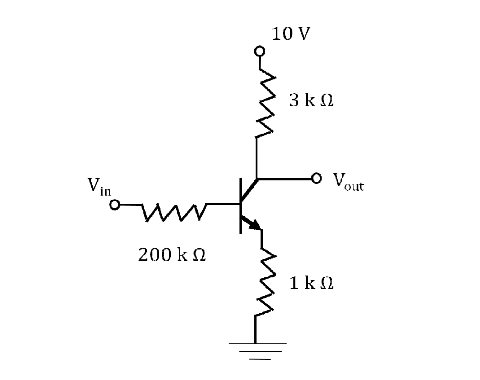
\includegraphics[width = 0.8\columnwidth]{fig/Q52.png}
    \caption*{}
    \label{fig:Q52}
   \end{figure}
    \item The state of a system is given by
    \begin{align*}
        |\psi\rangle = |\phi_1\rangle + 2|\phi_2\rangle + 3|\phi_3\rangle
    \end{align*}
    where $|\phi_1\rangle$, $|\phi_2\rangle$ and $|\phi_3\rangle$ form an orthonormal set. The probability of finding the system in the state $|\phi_2\rangle$ is \underline{\hspace{2cm}}. (Give your answer upto two decimal places)

    \item According to the nuclear shell model, the respective ground state spin-parity values of $^{15}_{8}\mathrm{O}$ and $^{17}_{8}\mathrm{O}$ nuclei are
    \begin{multicols}{2}
    \begin{enumerate}
        \item $\frac{1}{2}^+, \frac{1}{2}^-$
        \item $\frac{1}{2}^-,\frac{5}{2}^+$
        \item $\frac{3}{2}^-,\frac{1}{2}^+ $
        \item $\frac{3}{2}^- , \frac{1}{2}^-$
    \end{enumerate}
    \end{multicols}
  
    \item A particle of mass $m$ and energy $E$, moving in the positive $x$ direction, is incident on a step potential at $x = 0$, as indicated in the figure. The height of the potential is $V_0$, where $V_0 > E$. At $x = x_0$, where $x_0 > 0$, the probability of finding the electron is $1/e$ times the probability of finding it at $x = 0$. If $\alpha = \sqrt{\dfrac{2m(V_0 - E)}{\hbar^2}}$, the value of $x_0$ is
\begin{figure}[H]
    \centering
    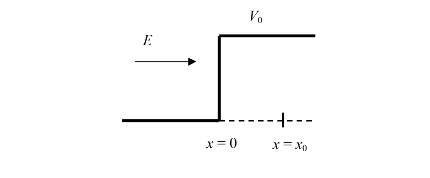
\includegraphics[width = 0.5\columnwidth]{fig/Q55.png}
    \caption*{}
    \label{fig:Q55}
\end{figure}
    \begin{multicols}{4}
    \begin{enumerate}
        \item $\dfrac{2}{\alpha}$
        \item $\dfrac{1}{\alpha}$
        \item $\dfrac{1}{2\alpha}$
        \item $\dfrac{1}{4\alpha}$
    \end{enumerate}
    \end{multicols}
    \section*{END OF THE QUESTION PAPER}





\end{enumerate}



    
\end{document}




